\documentclass[parskip]{cs4rep}

\usepackage{graphicx}
\usepackage{pseudocode}
\usepackage[T1]{fontenc}
\usepackage{amsmath}
\usepackage{algorithm2e}
\usepackage{array}

\begin{document}

\title{Plan Recognition in RISK}

\author{Jibran Abdus Zaahir Khan}

% to choose your degree
% please un-comment just one of the following
%\degree{Artificial Intelligence and Computer Science}
\degree{Artificial Intelligence and Software Engineering}
%\degree{Artificial Intelligence and Mathematics}
%\degree{Artificial Intelligence and Psychology }   
%\degree{Artificial Intelligence with Psychology }   
%\degree{Linguistics and Artificial Intelligence}    
%\degree{Computer Science}
%\degree{Software Engineering}
%\degree{Computer Science and Electronics}    
%\degree{Electronics and Software Engineering}    
%\degree{Computer Science and Management Science}    
%\degree{Computer Science and Mathematics}
%\degree{Computer Science and Physics}  
%\degree{Computer Science and Statistics}    

% to choose your report type
% please un-comment just one of the following
%\project{Undergraduate Dissertation} % CS&E, E&SE, AI&L
%\project{Undergraduate Thesis} % AI%Psy
\project{4th Year Project Report}

\date{\today}

\abstract{
This paper presents the design and implementation of a plan recognition agent based on an algorithm published by Christopher Geib and Robert Goldman in 2009 \cite{Geib:2009:PPR:1550966.1551246} called The Probabilistic Hostile Agent Task Tracker (PHATT). The plan recognition agents goal is to attempt to infer the unknown plan of a hostile agent from observations of their behaviour in the RISK environment.
}

\maketitle

\section*{Acknowledgements}

Michael for agreeing to supervise project, parents, family for support, C.Geib for advice and taking his time to meet with me, friends, people who helped with results

(Distinguish between academic and non-academic work.)

\tableofcontents

%\pagenumbering{arabic}

\chapter{Introduction}

\begin{flushleft}
\textit{AI has the potential to become the new driving force behind computer game innovation.}
\end{flushleft}
\begin{flushleft}
John David Funge, Artificial Intelligence for Computer Games, An Introduction
\end{flushleft}

\section{Motivations}

Artificial Intelligence for games or commonly termed 'game A.I.' has been an area of research ever since the beginning of significant work on A.I. Though techniques for game A.I. have typically come from academia and as John Funge argues \cite{JohnFunge:AIForComp} is notably different in both scope and application.

The primary goal of academia is to further human understanding often by solving particularly complex problems,as a result the scope of developed A.I. techniques from academia are usually more general in their application.

On the other hand game A.I. is built to provide an enjoyable experience for those playing the game, usually by creating the illusion of intelligence. Game A.I. is frequently built with a singular purpose in mind, which is generally considered to be any kind of control problem in a game.

Companies in the games industry who utilize game A.I. (which today is the vast majority) tirelessly seek an edge over their competition. This edge has typically come from computer graphics, effects such as dynamic rendering, the move from two dimensional to three dimensional to keep their customers interest. 

Emerging though is the idea that as users become accustomed to high quality graphics, developers will require something new to give their product an edge over their competitors. That edge will hopefully be better quality game A.I. and indeed there has already been examples of successful games acclaimed for their game A.I, one such is F.E.A.R. 

A First Person Shooter psychological horror video game, F.E.A.R utilizes a S.T.R.I.P.S. style planning-architecture which developer Jeff Orkin termed Goal-Oriented Action Planning, G.O.A.P. \textbf{[ref]}. \textbf{Talk briefly about what G.O.A.P. does.}

The game gained much acclaim and is commonly referenced as an excellent example of game A.I.

With this shift in focus, there grows greater incentives for developers to  and as a result more opportunities for the continued development of game A.I. likely as in the past with techniques developed in academia. Plan recognition algorithms may provide such an opportunity. 

Plan recognition is the problem of inferring an agents plans from observations. Research in plan recognition began in the 1980's, the results of which have been numerous applications in a variety of fields.

In Nate Blaylocks paper on "Retroactive Recognition of Interleaved Plans for Natural Language Dialogue" \cite{oai:CiteSeerPSU:538953} he highlighted a few of the most prominent applications of plan recognition as being:

\begin{tabular}{|l|p{8cm}|}
\hline 
\textbf{Field} & \textbf{Some Applications} \\ 
\hline 
User Modelling & Operating Systems, Intelligent Help Systems, Intelligent Tutoring \\ 
\hline 
Multi Agent Interaction & Military Tactical Defence, Multi Agent Coordination \\ 
\hline 
Natural Language Processing & Story Understanding, Machine Translation, Dialogue Systems \\ 
\hline
\end{tabular} 
\newline

Plan recognition continues to receive attention by various computer science communities due to its ability to both provide personalized responses, and an understanding that the consquences of failing to recognise plans, can in some situations be dire. Though not so much the latter point as losing video games is argueably trivial, applying plan recognition to games are no different.

Plan recognition has been used to perform automated game analysis, which potentially could be used to improve player performance. More exiciting though is the prospect of combining plan recognition algorithms with planning-architectures such as G.O.A.P. The result could be A.I. capable of recognising plans and subsequently building counter plans.

\section{Artificial Intelligence and Board Games}

In 1950 Alan Turing published a landmark paper "Computing Machinery and Intelligence" establishing the Turing test, marking what many consider to be the 'birth of Artificial Intelligence'. Soon after John McCarthy officially coined the term Artificial Intelligence at a conference in Dartmouth College. He defined it as "the science and engineering of making intelligent machines".

Thirty five years earlier Leonardo Torres y Quevedo had built "El Ajedrecista" a chess automaton[ref] capable of playing a king and rook endgame against a king from any position. It was considered the worlds first computer game and arguably the beginning of Artificial Intelligence and board games a relationship older than the term Artificial Intelligence itself. 

As AI continued to develop so did the complexity of the A.I's seen in computer games, first AI to appear which used enemies was arcade game [ref].

Since then notable achievements such as Garry Kasparovs defeat to IBMs chess computer Deep Blue in 1997 has continued to impress the public. 

From history it seems clear that AI and its application in games are intertwined becoming a growing area of interest in both commercial and academic fields.

Games are often considered a good metric for testing the quality of an AI [Ref].. 

Some academic work done on RISK in particular. Development of an Intelligent Artificial Player for the Game of Risk[ref]. The author Michael Wolf[ref] claims RISK is generally well known but under recognised by academia.

Work by two guys at Stanford on AI agent to play RISK, RISK as the intersection between traditional and modern board games.

\section{Aims}

What do we want to achieve?

To design a plan recognition agent for the board game RISK based on the PHATT algorithm developer by Geib and Goldman.

To implement a plan recognition agent for the board game RISK that can make successful predictions.

To further understanding of the complexities of performing plan recognition in the board game RISK.

\section{Objectives}

To show plan recognition algorithms can be used successfully to predict an agent's plan in the board game RISK with an accuracy better than randomly picking a mission card.

To provide insight into the complexities of creating plan recognition models for the RISK environment.

To provide insight into the nature of making plans in RISK. 

\section{Hypothesis}

What do you want to answer?

Are plan recognition algorithms beneficial in games? Specifically RISK?

If the player is a winner, then the prediction accuracy will be better.

If the probability of a mission card is the highest among all the other mission cards of an agent, then it will be the correct mission card.

Why because they are an artificially derived benefit which can be used by a player to optimize their behaviour, not solely , but in conjunction with the results of a plan recognition system.

Using more data from risk environment in the computation of the likelihood of explanations, the better the prediction accuracy will be.

\section{Paper Structure}

The structure of the paper is as follows:

The following chapter presents a background to the project where plan recognition and the board game RISK are introduced. Reasons for using plan recognition in board games are then discussed.

Chapter 3 describes the methodology of the project, it is split into two sections. The first is design, in this section PHATT is introduced and the design of the plan recognition agent is detailed. The subsequent section is implementation. Code related issues such as modifications to the open source project and any relevant design concepts are discussed. 

Finally an an evaluation plan and conclusion is presented. In these, the experimental findings are presented, discussed and any conclusions derived from the experimental findings are presented.

\chapter{Background}

\section{Previous Work in Plan Recognition}

Many consider one of the earliest projects on plan recognition to have been in 1978. Having identified plan recognition as a problem in itself, Schmidt et al \cite{journals/ai/SchmidtSG78} conducted experiments to determine whether or not people inferred the plans of other agents. From their results they created a rule based system called BELIEVER which attempted to capture the process of plan recognition. 

Three years later Cohen, Perrault and Allen identified two different types of plan recognition \textit{keyhole} and \textit{intended} \cite{Cohen82a}. 

They defined each as:

\begin{itemize}
\item
\textit{Keyhole plan recognition} is the recognition of an agent's plan through unobtrusive observation".
\item
\textit{Intended plan recognition} is the recognition of the plan of a cooperative agent who wishes to be understood.
\newline
\end{itemize}

In 1986 Kautz and Allen published a paper titled "Generalized Plan Recognition" \cite{conf/aaai/KautzA86} which set the frame work of many plan recognition projects that followed and formed the basis of plan recognition through logic and reasoning. They defined keyhole plan recognition as involving the identification of a set of top-level goals from possible plans, which could be decomposed into related sub-goals and basic actions, thus creating an event hierarchy also known as a \textit{plan library}. 

It was Charniak and Goldman \cite{journals/ai/CharniakG93} who first argued that plan recognition was largely a problem of reasoning under uncertainty and that any system which did not account for uncertainty would be inadequate. They went on to propose a probabilistic rather than logic based approach to  plan recognition using a Bayesian model. Their research continues to be popular in many avenues of research including its application in games.

Albrecht, Zukerman and Nicholson \cite{Albrecht98bayesianmodels} performed research on keyhole plan recognition using dynamic Bayesian networks to represent features of an adventure game. The result of their experiments they claimed "showed promise" for some domains. 

More recently Synnaeve and Bessiere \cite{conf/aiide/SynnaeveB11} published a paper of the design and implementation of a plan recognition agent that through observations of building construction in the game Starcraft, can predict the types of units a player intends to produce based on what buildings they construct.

\subsection{An Example of Plan Recognition}

We can introduce common concepts, assumptions and the process of plan recognition with an example of an agent attempting to infer the plan of another agent in a non-adversarial environment. 

Person A is cooking a meal for Person B, in other words A has a single \textit{root goal} (a state they wish to reach), such as cooked beef hamburgers. This root goal can be decomposed into a number \textit{sub-goals} of such as cook meat patties or \textit{actions} such as make meat patties  which can be further decomposed into single actions

A wanting to surprise B, will not tell B what his root goal is. B cannot know what A is thinking but B must then somehow infer what A's root goal is likely to be by \textit{observing} A cook in this way A's behaviour can be modelled as a Hidden Markov Model. Person B then models A's plan as follows. 

Person B assumes A is rational and that A has a \textit{plan} to achieve their root goal. Whatever A's root goal is, it can likely be decomposed into \textit{sub-goals} such as prepare burger buns or cook beef patties. These sub-goals can then be broken down into basic \textit{actions} to achieve those sub-goals, such as take beef patties out of packet. An important point to note is that these basic actions are not limited to only being part of a sub-goal.

To simplify the example, we introduce various assumptions:

\begin{itemize}
\item
A believes that they can cook a meal.
\item
B can only infer the cooking plan of A by observing what A is cooking.
\item
B knows everything that A can cook.
\item
Through observing A cook, B can predict with absolute certainty what A will cook.
\item
A cannot hide any observations.
\item
A only wishes to cook one meal.
\item
A has no preferences of what to cook, in other words given a choice the probability of choosing is equally likely.
\item
One A does not change cooking plan.
\end{itemize}

Given these assumptions and B's knowledge of A's cooking abilities we can model the set of all of As plans, following the notation set by Geib and Goldman in their paper on PHATT.

\begin{figure}[h]
\centering
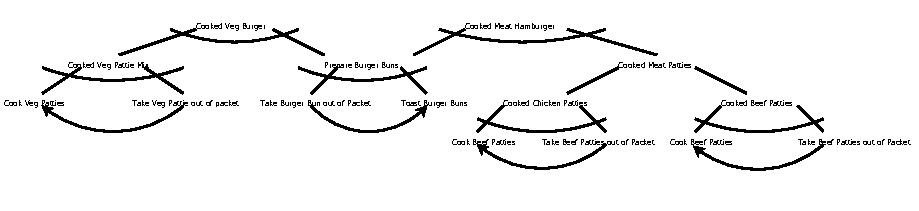
\includegraphics{images/example-plan-recognition}
\caption{Root goals are nodes that have no parent nodes. Sub-goals are nodes that have both a parent and children and actions are nodes that have no children. And-nodes are represented by an undirected arc across the lines connecting the parent node to its children. Or-nodes do not have this arc. Actions or goals that are dependant on a previous action are represented by an arc with an arrow.}
\label{fig:example-plan-library}
\end{figure} 

A top level or root goal is cooked vegetarian (veg) burgers, it is an and-node and this means that its children represent what needs to be done by A to accomplish that root goal. 

Children of or-nodes such as cooked meat patties represent options available to A to accomplish the goal. For example to achieve the goal cook meat patties A could either accomplish cooked chicken patties or cooked beef patties.

Arrows represent dependencies between nodes. For example to be able to accomplish the action cook beef patties, A must first perform the action Take Beef Patties out of packet.

Now A first performs the action \textit{Take Burger Bun out of Packet}, then proceeds to \textit{Toast Burger Buns}. At this point looking at the plan library we have two possible \textit{explanations} for As behaviour, cooked veg burger or cooked meat hamburger.

Each of these explanations are equally likely at this point because the actions that have occured so far could be part of either plan.

A then takes the Chicken Patties of their packet, now given our assumptions we can conclude that A's plan is to cook Meat burgers. In this way B has recognised A's plan thus performing the process of plan recognition.

\newpage

\section{Introduction to RISK}

Developed and released by french film director Albert Lamorisse in 1957 as La Conqu\^ete du Monde, RISK is a turn-based board game for two to six players. There exist many variations but the standard version, which this paper is concerned with, is an adversarial environment where players vie to control a fully observable board portraying a static geographical map of the Earth.

\subsection{Equipment}

\begin{figure}[h]
\centering
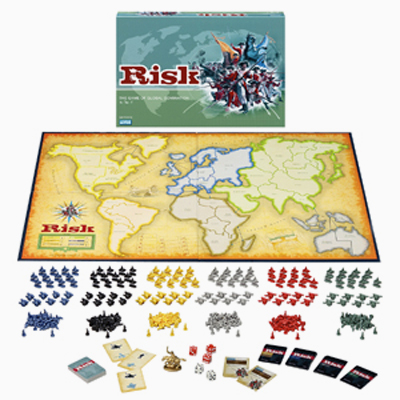
\includegraphics{images/risk-board}
\caption{Risk Equipment}
\label{fig:risk-equipment}
\end{figure}

The game consists of three pieces of equipment:

\begin{itemize}
\item
A board portraying a geographical map of the earth.
\item
Different coloured tokens called \textit{armies}.
\item
Two sets of regular six-sided dice.
\item
A deck of forty four cards.
\end{itemize}

\subsection{Rules}

The board is divided into forty two \textit{territories}. Each territory is a representation of a real country on Earth. These territories are partitioned into six \textit{continents} usually corresponding to their real continent grouping.

For each territory is a corresponding card, in addition to the name of that territory each card either depicts the symbol of an infantry, cavalry or artillery. By successfully occupying another player's territory in a turn, a player is then award a card and no more than one in that turn. Additionally there are two wild cards which can be substituted to represent a symbol of the players choosing.
Owning a set of three cards with the same symbols or a set of three distinct symbols gives the player the opportunity to trade the set of cards for additional armies.

Armies are placed in territories. If a player places an army in a territory, this declares that the player \textit{occupies} that territory. Players must have at least one army placed in a territory they own at all times. Players can choose to place as many additional armies as they wish in that territory.

How a player wins largely depends on the \textit{Game mode}. Game modes significantly impact the behaviour of players and is decided by players beforehand. In standard RISK they are:
\newline

\begin{tabular}{|l|p{11cm}|}
\hline 
\textbf{Game Mode} & \textbf{Description} \\ 
\hline 
Domination & Players aim to conquer a certain number of territories, \\ 
\hline 
Mission & Each player is given a single unique mission card. A mission card describes a state they must reach e.g. Occupy North America and Africa, for the rest of the game this is their \textit{root goal} which only they know. In order to win they can either complete this root goal or eliminate all other players. \\ 
\hline 
Capital Risk & Each player is given a Capital territory and to win a player must occupy all other Capital territories. \\ 
\hline
\end{tabular} 
\newline

This paper is concerned with the mission game mode \textbf{only}, therefore the following sections describe rules only for that game mode.

After an initial setup, each player's turn is split into three distinct phases which always occur in the same fixed order. These phases are:

\begin{enumerate}
\item
Reinforcement
\item
Attack
\item
Movement
\newline
\end{enumerate}

In each phase a player performs atleast one discrete \textit{action} which helps to further the players goals, thus forming a sequential task environment.

\subsubsection{Initial Setup}

The game begins with an an initial setup, it involves:

\begin{itemize}
\item
Territories being divided equally between players.
\item
Players being given a starting number of armies which is inversely proportionally to the number of players.
\item
Players distributing their starting armies over their territories.
\item
Each player being given a mission card.
\end{itemize}

\subsubsection{Reinforcement Phase}

At the start of a player's turn, they receive \textit{reinforcements} in the form of additional armies. The act of placing an army in a territory is called \textit{reinforcement}.  The number of additional armies received is based on the number of territories a player occupies and whether they occupy any continents.
\newline

\begin{table}[ht]
\centering
\begin{tabular}{|c|c|}
\hline 
\textbf{Occupied Continent} & \textbf{Number of Bonus Armies} \\ 
\hline 
Asia & 7 \\ 
\hline 
North America & 5 \\ 
\hline 
Europe & 5 \\ 
\hline 
Africa & 3 \\
\hline
Australia & 2 \\
\hline  
South America & 2 \\
\hline 
\end{tabular}
\caption{Occupied Continent Army Reinforcement Bonus}
\label{table:continent-bonus}
\end{table}

\subsubsection{Attack Phase}

Once a player has distributed their armies from the reinforcement phase, they can choose to \textit{attack}. 

Territories occupied by a player that contain more than one army can attack neighbouring territories occupied by any other player. An attack consists of several \textit{battles}. The outcome of a battle is decided by means of rolling two sets of dice, thus making it a stochastic environment. One set is rolled for the \textit{defender} of the territory and the other for the \textit{attacker}. 

The number of dice each player receives for a battle is dependant on the number of armies placed in each of the players respective territories. The defender receives a die per army up to two armies. The attacker receives a die per army upto three armies not including the single army they are required to have in that territory while occupying it. 

The general rules of engagement are, dice rolls of each player are compared on a one to one basis in descending order of values. The player with the lower value at each comparison loses a single army, if the die are equal the attacker loses an army. The number of comparisons per battle are set by the number of dice the defending player has rolled. The attacking player can commence as many battles as they wish during an attack provided they have more than one army in the attacking territory.

An attack of a territory has three outcomes:

\begin{itemize}
\item
A \textit{failedAttack} by the attacker as they have only one army remaining in which case they must retreat and a \textit{successfulDefence} by the defender who retains the territory.
\item
A \textit{failedAttack} by the attacker as they choose to retreat before having only one army remaining and a \textit{successfulDefence} by the defender who retains the territory.
\item
A \textit{successfulAttack} by the attacker who occupies the territory and a \textit{failedDefence} by the defender who has no armies remaining and so loses the territory. The attacking player, leaving atleast one army behind, must then move armies from the territory they attacked from into the newly occupied territory.
\end{itemize}

A player can perform any number of attacks from any territory they own during their turn, provided they have more than one army in the territory they choose to attack from.

\subsubsection{Movement Phase}

When either the player chooses to end the attacking phase or can no longer attack because they do not occupy a territory which contains more than one army their movement phase begins.

During their movement phase a player may move armies from one territory to an neighbouring territory they own, provided they leave atleast one army in the territory the armies were moved from. This action can only be done once per turn in this phase, after which the movement phase is finished.

After the movement phase has been completed the players turn ends and another players reinforcement phase begins.
\newpage

\section{Why Plan Recognition in Board Games}

Algorithmic landmark - such as the solution of the game of checkers 

In the realm of board games such as chess, there have for many years dominated a number of algorithms such as the:

Min-max Algorithm with Alpha-Beta Pruning

Many games today have a large number of alternative moves are stochastic and have hidden state attributes. "Applying traditional game tree search algorithms designed for perfect information games that act on the raw state representation is infeasible" [ref Monte Carlo Planning in RTS Games], this has been said because the search space for such games is large and that finding the best move would take an unreasonable amount of time (Find a ref for this) Michael Wolf paper calculating state space for RISK is infinite.

Instead of a brute force method of finding the best alternative the idea of plan recognition offers another method. Use plan recognition algorithms one can weed out unlikely explanations before committing to a search of the 

Main benefit is that responses can be personalized.

This issue prompted research into the development of variants of the original algorithms that could cope but this 

Using these algorithms people like Kabanza are starting to be able to tackle certain aspects which are harder to model?

\section{Summary}

\chapter{Design}

\section{Introduction to PHATT}

PHATT was published by Christopher Geib and Robert Goldman in 2009. In their paper they presented the central realization of PHATT's approach being "that plans are executed dynamically and the actions that an agent takes at each step depend critically on the actions that the agent has previously taken". 

They introduced a model of plan execution based on the notion of \textit{pending sets} of actions. A pending set is what actions an agent can take based on actions it had already performed, calling it "actions that are pending execution by the agent".

Plan execution according to PHATT was modelled as the following. An agent would first choose a root goal, then a set of plans to achieve that root goal. Any actions of those plans that had no pre-requisite actions would form the initial pending set of the agent. The agent would then perform an action from the initial pending set and this would result in some actions being appended to the pending set and others being removed to form a new pending set. The agent would then continue to perform actions until an outcome such as, the agent concluding the root goal had been achieved.

From this model of plan execution, Geib and Goldman proposed an algorithm utilizing a Bayesian approach to perform probabilistic plan recognition. It computed \textit{Pr(g}|\textit{obs)}, the conditional probability of a goal \textit{g} given a set of observations \textit{obs}, by computing \textit{Pr(exp}|\textit{obs)}, the conditional probability of a particular explanation \textit{exp} of the likelihood of an agent having that root goal, given a set of observations \textit{obs}.

Using Bayes Rule they defined \textit{Pr(exp}|\textit{obs)} as:\newline

\centerline{
\textit{Pr(exp}|\textit{obs)} = \textit{Pr(exp} $\wedge$ \textit{obs)} / \textit{Pr(obs)}
}

They then (as other practical Bayesian systems do) exploited the equivalent formulae\newline

\centerline{
\textit{Pr($exp_0$}|\textit{obs)} = \textit{Pr($exp_0$} $\wedge$ \textit{obs)} / $\displaystyle\sum\nolimits_{i}$ \textit{Pr($exp_i$} $\wedge$ \textit{obs)}
}

This they described as the conditional probability of the explanation $exp_0$ being computed by dividing the conditional probability of $exp_0$  by the sum of the probability mass associated with all possible explanations.

\subsection{Computing an Explanation's Probability}

To compute the term \textit{Pr(exp} $\wedge$ \textit{obs)} requires the plan library to be augmented with three probabilistic features:\newline

\begin{enumerate}
\item
The prior probability of the root goal.
\item
The respective probabilities of choosing any sub-goals.
\item
The probabilities of picking actions from the agents pending set.\newline
\end{enumerate}

The probability of an explanation is then calculated by multiplying each of the terms together in the following manner: \newline

\centerline{
\textit{Pr(exp} $\wedge$ \textit{obs)} = \textit{P}(\textit{goals})\textit{P}(\textit{plans}|\textit{goals})\textit{P}(\textit{obs}|\textit{exp})
}

\section{Environment Modelling}

\subsection{Root Goals}

The root goals of the RISK environment are the mission cards, these are:

\begin{itemize}
\item
Occupy Europe, Australia and one other continent.
\item
Occupy Europe, South America and one other continent.
\item
Occupy North America and Africa.
\item
Occupy North America and Australia.
\item
Occupy Asia and South America.
\item
Occupy Asia and Africa.
\item
Occupy 24 territories.
\item
Occupy 18 territories and occupy each with atleast two troops.
\item
Eliminate a player.
\newline
\end{itemize}

A subset of these where the mission involved occupying continents were chosen to be the focus of this paper. These mission cards are of two types:

\begin{enumerate}
\item
\textit{Two-Continent}: Players must occupy two explicitly named continents.
\item
\textit{Two-Continent+1}: Players must occupy two explicitly named continents and another of their choice.
\end{enumerate}

As mission cards are handed out at random, the prior probability of a root goal is 1/$n$ where $n$ is the number of mission cards. The data structure of a root-goal is in the form of a tuple containing the name of the root goal and its prior probability.

\centerline{
 $RG$ = \{ rootGoalName, 1/$n$\} .
}

\subsection{Sub-Goals}

The root goals of the RISK environment can be decomposed to form a set of sub-goals. 

\begin{itemize}
\item
For \textit{Two-Continent} root goals, the sub-goals of that root goal are occupying each continent. 
\item
For \textit{Two-Continent+1} root goals which requires players to allow an option to occupy a continent of choice, provided they also occupy two explicitly named continents. 
\end{itemize}

These two types of root goals therefore make the occupation of any single continent a sub-goal of atleast one root goal. The prior probability of a sub-goal is modelled as 1/$c$ where $c$ is the number of alternate sub-goals available in an explanation. The data structure of a sub-goal is a tuple containing the name of the sub-goal and the probability associated with choosing that sub-goal.\newline

\centerline{
 $SG$ = \{ subGoalName, 1/$c$\} .
}

\subsection{Actions}

Excluding card related actions, in RISK the only actions players perform are:

\begin{itemize}
\item
Attacking a Territory.
\item
Defending a Territory.
\item
Occupying a Territory.
\item
Losing a Territory.
\item
Reinforcing a Territory.
\item
Moving armies into a Territory.
\item
Moving armies out of a Territory.
\end{itemize}

Each of these action must be modelled in a manner that contributes towards explanations of a player's behaviour.

\subsubsection{Attacking}

Though players can perform several attacks during their turn, they can only attack one territory at a time. Thus players' must choose what territory to attack and, if they wish to attack additional territories, in which order to attack provided they have neighbouring territories and sufficient armies. Modelling these choices provides an avenue to infer a players plan.

The pending set of a player's attack actions for any turn is to either successfully or unsuccessfully attack territories they do not own, that are neighbour to atleast one territory that they own which also contains atleast two armies.

If a player $p$ successfully occupies a territory $T_{o}$, then the attack actions of neighbouring territories of $T_{o}$ are added to $p$'s attack pending set. If they lose a territory $T_{l}$ due to another players successful attack, then any attack actions of neighbouring territories of $T_{l}$ are removed from their attack pending set for their next turn. 

The attack action is thus modelled as a singular event that is either \textit{consistent} or \textit{inconsistent} with explanations of a players behaviour.

For example, given three explanations:

\begin{enumerate}
\item
Occupy North America and Australia.
\item
Occupy North America and Africa.
\item
Occupy Asia and South America.
\end{enumerate}

Successfully occupying a territory in North America would be consistent with explanations 1 and 2, but inconsistent with 3, or in probabilistic terms the likelihood of 1 and 2 would rise whereas 3 would fall.

Having defined the outcome of attacks as either successful or unsuccessful, attacks can be decomposed into following two actions: 

\begin{table}[ht]
\centering
\begin{tabular}{|c|c|p{8cm}|}
\hline 
\textbf{Action} & \textbf{Consistent}  & \textbf{Reasoning} \\ 
\hline 
SuccessfulAttack & Yes & A good indication of a players plan is the territories they attack and successful attacks are in themselves the best outcome. \\ 
\hline 
FailedAttack & Yes & Though less significant than a successful attack, attacking a territory is indictive of a players intention to occupy that territory and therefore a consistent action with an explanation.\\ 
\hline
\end{tabular}
\caption{Modelling Attack Actions}
\label{table:attack-defend-modelling}
\end{table}

\newpage

\subsubsection{Defending}

Defending as opposed to attacking can be seen as a 'passive' action as an attack is required before a defence can occur. In that way defence can be modelled as only inconsistent with the explanations it is directly related to and, as an act in itself, not related to those it is not. 

Practically this is difficult to achieve given the nature of competing explanations, but by making the probability term of representing a defence action large then this effect can be atleast minimised.

For example, given the three explanations from the previous section. If a successful defence were to occur in a territory in North America explanation one and two could be multipled by 1.01. If a failed defence were to occur then explanations one and two would be multiplied by 0.99. This would model a change in the likelihood of both explanations and should have a comparatively minimal effect on the likelihood of explanation 3. 

Defence in the same manner as attack can be either successful or unsuccessful, therefore defence can also be decomposed into the following: 

\begin{table}[ht]
\centering
\begin{tabular}{|c|c|p{8cm}|}
\hline 
\textbf{Action} & \textbf{Consistent}  & \textbf{Reasoning} \\ 
\hline 
SuccessfulDefence & Yes & A successful defence of a territory may be purely based on chance, but is more likely when a player has invested armies in the defence of that territory and so observing the action provides a sign that they have an plan involving that territory. \\ 
\hline 
FailedDefence & No & An inconsistent action because a player would not normally allow a territory to be lost if it is a part of their plan. \\ 
\hline
\end{tabular}
\caption{Modelling Defence Actions}
\label{table:attack-defend-modelling}
\end{table}

\newpage

\subsubsection{Reinforce}

The reinforce actions that a player $p$ can perform at any turn $t$ is based solely on the territories that $p$ owns during turn $t$. The pending set of any players reinforce actions is therefore modelled as follows. 

For each territory $T$ that $p$ owns at a certain turn $t$. In $p$'s pending set is an action to reinforce $T$. If a territory $T_{l}$ is lost by $p$ (it is attacked then occupied by another player), its corresponding reinforce action is removed from the players pending set for the players turn at $t+1$. Conversely if another territory $T_{o}$ is occupied by $p$ then a reinforce action for $T_{o}$ is added to the players pending set at turn $t$.

\subsubsection{Movement}

The pending set of movement actions of player $p$ is the set of territories a player owns that are neighbour to a territory where $p$ has more than one army. Moving armies into a territory is modelled as a consistent action with the explanation that the territory that had armies moved into is directly related to.

\subsection{Territory}

Each territory is modelled as an entity. When a player occupies a territory the player gains access to a set of actions which together form that territories action set.

The action set of any territory is:

\begin{table}[ht]
\centering
\begin{tabular}{|c|c|}
\hline 
\textbf{Action} & \textbf{Description} \\ 
\hline 
SuccessfulAttack & Attacking and occupying the territory.\\ 
\hline 
FailedAttack & Attacking and failing to occupy the territory.\\ 
\hline 
SuccessfulDefence & Retaining the territory after an attack.\\ 
\hline 
FailedDefence & Losing the territory due to an attack.\\
\hline
Movement & Moving armies in to the territory.\\
\hline  
Reinforce & Placing armies in the territory.\\
\hline 
\end{tabular}
\caption{Territory Action Set}
\label{table:continent-bonus}
\end{table}

\newpage

The data structure of a territory therefore is a triple containing the name of the territory the set of territory actions  $TA$ and a set of references to the territories neighbours $TN$.

\centerline{
$T$ = \{ territoryName, $TA$, $TN$ \} 
}

A key concept in the design of the agent is that the pending set of a player is decided \textit{a priori} as it is based on the territories a player owns. By combining the action sets of each territory a player owns into a single set, all the actions a player can perform can be captured.

\subsection{Continent}

Each continent contains atleast two territories and so can be modelled as a tuple of the name of the continent and the set of territories that are contained in that continent.

\centerline{
$C$ = \{continentName, <$T_{1}$ ... $T_{n}$>\}
}

\subsection{Player}

The term player has been and can be used inter changeably with the term agent. A defined data structure for a player is essential to be able to separate the numerous explanations of one player from another. The data structure must contain alteast three features. A player name or ID, a list of territories they own $PT$ and a list of explanations $PE$.\newline

\centerline{
$P$ = \{playerName, $PT$, $PE$\}
}

\section{Explanations}

Explanations must be designed to contain all the necessary data required to compute its probability, it therefore contains these features:

\begin{itemize}
\item
The explanation name.
\item
A root goal $RG$.
\item
A set of sub-goals $SGS$.
\item
A set of consistent actions $ECA$.
\item
A set of inconsistent actions $EIA$.
\end{itemize}

The resulting data structure is:\newline

\centerline{
$E$ = \{ explanationName, RG, SGS, ECA, EIA \}
}

Inconsistent actions are stored in explanations due to modelling decisions as if it was the case that that if an action is not consistent then it is inconsistent then defence actions would be modelled incorrectly. Defence actions are not considered inconsistent to explanations that they are not directly related to, but would be if any actions not in the set of consistent actions are classified as inconsistent actions to an explanation.

Explanations of the form Two-Continent+1 have four alternate forms. For example the root goal Occupy Europe, South America and one other continent can be any of the following:

\begin{itemize}
\item
Occupy Europe, South America and Asia.
\item
Occupy Europe, South America and Africa.
\item
Occupy Europe, South America and North America.
\item
Occupy Europe, South America and Australia.
\end{itemize}

Each is a valid explanation in itself, but still falls under its parent mission card. Therefore the assumption is made that if the plan recognition agent predicts one of the four children when it is known the players mission card is the parent, it is classified as a correct prediction.

Given the list of root goals and sub-goals, the complete list of explanations is:

\begin{itemize}
\item
Occupy Europe, Australia and Africa.
\item
Occupy Europe, Australia and North America.
\item
Occupy Europe, Australia and South America.
\item
Occupy Europe, Australia and Asia.
\item
Occupy Europe, South America and Asia.
\item
Occupy Europe, South America and Africa.
\item
Occupy Europe, South America and North America.
\item
Occupy Europe, South America and Australia.
\item
Occupy North America and Africa.
\item
Occupy North America and Australia.
\item
Occupy Asia and South America.
\item
Occupy Asia and Africa.
\end{itemize}

Each of these are considered as possible explanations of a players behaviour. A design modification to PHATT follows this modelling choice. By unpacking (fully enumerating) each explanation, then assigning the full set of explanations to each player from the start of the game, the element of choice has been effectively removed. 

What is then measured is the probability of each separate explanation of a players behaviour over the course of the game.

\subsection{Prediction Agent Pseudo Code}

\subsubsection{Building the Set of Explanations}

During the initialisation of the RISK map, a set of explanations must be built for the environment to be later assigned to players. This require the explicit specification of a root goal and sub-goals for each explanation in the environment. In addition it also requires populating each explanation with a set of consistent and inconsistent actions, this can be done by the following operation:

\begin{pseudocode}[ruled]{generateExplanationList}{-}
\begin{algorithm}[H]
\ForAll {C $\in$ CS}{

	\ForAll{E $\in$ ES}{

		\If{C \textit{isSubGoalOf} E}{

			\ForAll{T $\in$ C}{

				\textit{addAction}(ReinforceT) to \textit{ECA}

				\textit{addAction}(MovementT) to \textit{ECA}
				\textit{addAction}(SuccessfulDefence) to \textit{ECA}
				\textit{addAction}(FailedAttackT) to \textit{ECA} \newline

				\textit{addAction}(FailedDefenceT) to \textit{EIA}
			}
		}
	}
}
\end{algorithm}
\end{pseudocode}

The above pseudo code loops through the data structure of each continent $C$ in the set of continents $CS$. Each continent is checked against each explanation $E$ from the set of explanation $ES$, for whether its name is contained in the set of sub-goals of each $E$ by the \textit{isSubGoalOf} operation. If true then the result is in an If statement firing. 

The If statement contains a loop which iterates over the set territories in the current loops continent and using the \textit{addAction} operation, adds each territories action set to the explanations to either the explanations consistent action \textit{ECA} set or inconsistent action set {EIA}.

\subsubsection{Generating Pending Sets}

With the set of environment explanations $ES$, each player is allocated a unique instance of each explanation. Since the computation of the probability of an explanation requires the probability of choosing an action, a function is required which generates a complete set of the available actions a player can perform.

\begin{pseudocode}[ruled]{generatePendingSet}{PT}
\begin{algorithm}[H]
\textit{playerPS} = $\emptyset$

\ForAll {T $\in$ PT}{

	\textit{addAction}(ReinforceT) to \textit{playerPS}

	\textit{addAction}(FailedDefenceT) to \textit{playerPS}

	\textit{addAction}(SuccessfulDefence) to \textit{playerPS}

	\ForAll{N $\in$ T}{
			
		\eIf {playerOwnsN}{

			\textit{addAction}(MovementT) to \textit{playerPS}
		}{

			\textit{addAction}(FailedAttackT) to \textit{playerPS}
			\textit{addAction}(SucessfulAttackT) to \textit{playerPS}
		}
	}

	\Return{playerPS}
}
\end{algorithm}
\end{pseudocode}

After initializing an empty pending set $playerPS$. The above pseudo code first loops through each territory $T$ in the list of all the territories that a player owns $PT$. For each territory a $ReinforceT$ action and a $LoseT$ action is added to $playerPS$. 

Before proceeding onto the next territory in $PT$ another loop is performed through the set of neighbouring territories $TN$ of that territory with an if-then-else statement. If the player owns that territory a $MovementT$ action is added to $playerPS$, if not then a $OccupyT$ action is added to $playerPS$. After the operation the $playerPS$ is returned and can be cached if necessary.

\newpage

\subsubsection{Computing Action Probabilities}

Following an idea from a paper by Goldman, Geib and Miller \cite{Goldman99anew} which proposes weighting actions, a method for assigning probabilities to pending set actions generated by the $generatePendingSet$ operation was used. It required an operation that would allow greater control over weighting between consistent and inconsistent actions.

\begin{pseudocode}[ruled]{ComputeBaseWeight}{w, playerTotalActNum, playerConsActNum}
\begin{algorithm}[H]

$sumWeight$ = $w$ * $consActNum$

$leftOver$ = 1.0 - $sumWeight$

$base$ = $leftOver$ / $totalNumAct$

\Return base
\end{algorithm}
\end{pseudocode}

Given a predefined weight $w$, the total number of actions in a players pending set $playerTotalActNum$ and the consistent actions with an explanation $playerConsActNum$. This operation computes a $base$ weight for all actions by subtracting the total weight of the desired actions from 1, then distributing equally the remainder amongst all the actions in the players action set. This operation could easily be replaced with another such similar method.

Given the nature of the environment where the number of actions players can perform are relatively small, this method is suitable provided the weight difference is kept small. For environments where the number of consistent or inconsistent actions a player can perform are large, this may result in the value of \textit{sumWeight} becoming greater than one making \textit{leftOver} negative, breaking the next calculation. Therefore a scalable method of controlling the weights between actions would be necessary in the design of such an agent for a larger action environment.

The operation $ComputeBaseWeight$ is part of a larger function which prepares the values which $ComputeBaseWeight$ requires.

\begin{pseudocode}[ruled]{ComputeObsProb}{playerPS, totalExpConAct , obs}
\begin{algorithm}[H]
$expConsAct$ = \textit{filterPS}(totalExpConsAct, actType) \newline
$playerTotalAct$ = \textit{filterPS}(playerPS, actType)\newline
$playerTotalActNum$ = size of playerTotalAct \newline

\textit{playerConsAct} = $\emptyset$ \newline

\ForAll{A $\in$ \textit{playerAct}}{
			
	\If {A $\in$ \textit{expConsAct}}{

		\textit{addAction}(A) to \textit{playerConsAct}
	}
}

playerConsActNum = size of playerConsAct\newline

base = \textit{computeBaseWeight}(w, playerTotalActNum, playerConsActNum)\newline

\Return base

\end{algorithm}
\end{pseudocode}

Given the players pending set $playerPS$ generated by the function $generatePendingSet$, and the set of all consistent actions for an explanation $totalExpConAct$. Both the set of actions (must be of the type $obs$) a player can currently perform $playerTotalAct$ and the consistent actions of the explanation can be be filtered using the $filterPS$ operation which given an action type ad a set, removes all other action types from the given set except for actions of the type specified. 

The set of $playerTotalAct$ is then further filtered down into another set $playerConsAct$ which contains only the consistent actions with the explanation. The sizes of $playerConsAct$ and $playerTotalAct$ are saved in two respective variables $playerConsActNum$ and $playerTotalActNum$.

Dividing these two variables effectively gives the proportion of available actions that a player can perform that are inconsistent and this fact is exploited by the next operation which is passed a predetermined weight and each variable to the $computeBaseWeight$ operation which returns the $base$ weight of an action. This base weight can easily be used to weight either inconsistent actions or consistent actions.

This formulae makes three assumptions:

\begin{enumerate}
\item
That any territories including ones that only contain one army can attack. Though this is not technically true, due to the nature of RISK where players are not restricted in any way on where they may place their armies during the reinforcement phase a player can practically attack any territory they do not own but have a territory they own neighbour to it at the start of their turn.
\item
That the likelihood of consistent attack actions are uniformly distributed.
\item
That the likelihood of inconsistent attack actions are uniformly distributed.
\end{enumerate}

\subsubsection{Computing Explanation Probabilities}

\begin{pseudocode}[ruled]{ComputeExplanationProbability}{explanation, obs}
\begin{algorithm}[H]

\If{\textbf{not} alreadyIni}{ 

	\textit{expProb} = 1.0

	\textit{expProb} = \textit{R} * \textit{expProb}	
}

\textit{playerPS} = \textit{generatePendingSet()} \newline

$weight$ = arbitrary number

$base$ = $computeObsProb$(playerPS, totalExpConsAct, obs)\newline

$conActProb$ = $base$ + $weight$

$inConActProb$ = $base$ \newline
Investment
\uIf{obs is consistent }{

	\textit{expProb} = $conActProb$ * \textit{expProb}	

	
}\ElseIf{obs is inconsistent}{

		\textit{expProb} = $inConActProb$ * \textit{expProb}

 }

\textit{expProb} = $normalized$(expProb)

\Return{expProb}
\end{algorithm}
\end{pseudocode}

After initialising the float $expProb$ the explanation is multiplied by the root goal prior $R$, this is done only when the explanation is initialised and therefore the $alreadyIni$ flag is necessary. To complete the computation of an explanation, the operation $computeObsProb$ is applied to $obs$. Depending on whether $obs$ is consistent or not with the explanation, the appropriate action probability is multiplied with $expProb$ .

Normalizing the explanation probability at the end of each operation is vital as this prevents the probability of any explanation from dropping to zero very quickly. 

\subsection{Example of Operation}

These concepts from this chapter can be tied together with an arbitrary example.

As mission cards are handed out to players' at random, the prior probability of each root goal is 1/\textit{n} where \textit{n} is the number of mission cards.

As we know the probability of being a mission card is uniform and though there are six mission cards, two of those have four derivatives resulting in 12 explanations of a players behaviour. Therefore the probability of a single explanation is 1/12.

Introducing some other assumptions for this example:

The probability of a player choosing to attack any territory is uniform.
The probability of a player choosing to occupy a continent as a sub-goal is uniform.
The RISK map has every territory connected a with every other territory.

Follow example in slides.

\subsection{Conceptual Issues}

Main change is that PHATT works in an action space whereas I have had to adapt the implementation to represent the state of the 'risk world' for the algorithm to operate.

Another difference is that I do not store or manipulated derivative trees as the original paper includes in the pseudo code it presents, this is due to hard coding derivative trees into explanations.

Another difference is I have removed the need for sub goal probabilities because of working with the full derivative tree.

Normalising after each observation computation rather than only when a probability needs to be computed.

Using the constraints in the environment initially the model was based on the plan library proposed in the PHATT paper. This was not good therefore utilized the constraints of countries to narrow the number of possible explanations and actions.

Initially the movement model was based on the attack model where the smaller the number of actions the bigger the weighting should be, this is an incorrect model as the number of territories a player owns increases as a player gains more consistent movement and reinforce actions as they continue to be successful in their goal.

\subsubsection{Probability Assignment}

Simple weighting based on reasoning about implications of an action to an explanation

Positively weighted probabilities towards consistent actions and negatively towards inconsistent actions

Uniform distribution

Weighting based on number of consistent and inconsistent actions available to a player when an action is performed.

Question was how to assign weights to consistent and inconsistent actions?

Total number of actions are counted, and are separated into inconsistent actions and consistent actions and a weight is split among inconsistent actions and consistent actions. Problem is that it seems this system is too sensitive.

Because of sensitivity had to make up a more evenly weighted automatic system.

Therefore made proportional weighted system

\subsection{Summary}

The summary for this section is

\chapter{Implementation}

Built purely in the Java programming language, the plan recognition agent follows an \textit{event-driven} system architecture.

THIS SECTION NEED TO BE LOOKED AT!

Diagram 

(Game -> Processing -> Events -> Plan Recognition Agent)

\textit{Game} represents an existing open source project of the board game RISK. Developed by Yura.Net, a team based in London headed by Yura Mamyrin the project is written in the Java programming language[ref - to website].

\textit{Event} objects contain important data from the environment which the plan recognition agent requires to compute the likelihood of explanations. 

The plan recognition agent needs to simply be aware of when the game beings, the changes that occur in the game state and when the game is finished. These \textit{events} are registered by the processing class and sent to the plan recognition agent.

Modifications to the project were minimal. Modifications such as:

Initialising the plan recognition agent and processing class when the game begins.

Statements that created events objects at the following key points in the \textit{Game}:

\begin{itemize}
\item
Player Initialisation
\item
Player Removal
\item
Territory Occupation
\item
Attacks
\item
Army Movements
\end{itemize}

Once fired these events are handled by a \textit{processing} class which (routes?) each event object to the plan recognition agent where it is handled in a manner depending on the event.

In this way the implementation of the plan recognition agent is not as a dependant sub-component of the game but rather a completely separate entity that operates in \textit{parallel} to the game.

Initially the plan recognition agent would store its own copy of the data structures from the RISK environment. Treated the game as a black box where only the changes in game state would be observable.

Agent data was generated such as countries they owned.
Agent explanations computed by the plan recognition agent based on events from the environment.

The reason for this choice was the simplicity of its implementation at the time and to reduce the dependence on the implementation of the project.

\section{System Construction}

(Diagram of data structure of local copy)

Adding data to this hard coded data structure proved to be overly time consuming and therefore was changed to an automated system of the generation of a data structure allowing the plan recognition agent to work on any RISK map that could be successfully played in the open source game.

Through the modelling process it is apparent that there is no need for the plan recognition agent to hold its own copy of the game state which is update via registration of events in the original code.

It could utilize the data structures from the game itself rather than storing a copy within the plan recognition agent.

This gives advantages such as less overhead and eliminating the possibility of the plan recognition agents local copy to lose sync with the actual game state. The disadvantage is that this makes the agent more dependant on the methods of the developers implementations.

Piggybacked off the games data structures and just inserted code into the project which registered events occurring in the main game.

\section{System Architecture Concepts}

\subsection{Google Guava Libraries}

The plan recognition agent makes extensive use of the freely available Google Guava libraries to allow the prediction agent to operate concurrently with the game as well as more efficiently in its operations.

\subsection{Replaying Games}

Used an inbuilt tool by the developer of saying "Debug Logs" which could be used to reproduce a game exactly, this allows the algorithm to be tested with different parameters on the exact same game thus ruling out any environmental difference when analysing data.

\section{Summary}

\chapter{Evaluation} 

1) Does it work?

It performs better than randomly guessing but still at a low probability

2) If not why?

Three types of games to test the algorithm in:

\section{Experiments}

\subsection{A.I. Play}

The RISK project has a built in A.I. for various game modes in particular it has one mission game mode. The A.I can be substituted for players to the point where a game can consist of upto six A.I. fighting each other completing a game in a fraction of the time compared to people. Monitoring these games provide an opportunity for the collection of a large number of data samples for testing the performance of the plan recognition agent.

\subsection{Constrained Play}

In this form of play, players are asked only to perform actions that are directly consistent with their root goal. This means for example players may not break another players continent even though preventing other players from completing their mission is in-directly consistent with completing a players own mission.

More formally this is defined as. Given a set of actions a player will only either:

\begin{itemize}
\item
Choose to attack a territory that is directly consistent with their plan or a territory that is on the shortest route to a territory that is directly consistent with their plan.
\item
Reinforce a territory that is directly consistent with their plan or a territory that is on the shortest route to a territory that is directly consistent with their plan.
\item
Moves armies to a territory that is directly consistent with their plan or a territory that is on the shortest route to a territory that is directly consistent with their plan.
\end{itemize}

By creating an artificially constructed form of play, this is clearly the easiest to perform plan recognition on and by establishing that the algorithm works given that players behave only a consistent manner with the mission they have been given.

\subsection{Free Play}

Free play can be easily described as players are simply "play to win". In this manner it should be exactly how players normally play mission RISK.

\section{Experimental Format}

There were two experiment formats, one for constrained play, the other for free play. But before either the rules of the game were explained to participants. 

For constricted play, the particular play style required was described to participants in detail

For free play it was made clear to participants that there were two primary methods of winning in mission risk. Either by eliminating all other participants from the game or by completing their mission card. The mantra was "Play to Win".

At the end of the game participants gave a short summary of their initial plan during the placement phase and any changes in plan from that during the course of the game.

\section{Data Collection}

After a game has finished the system generates two files. One a log file which using a debug tool created by the developers allows an exact replay of the game. 

This has significant implications in that the environment can be eliminated as a changing variable in the evaluation process. Since a game can be reproduced but with the plan recognition agent being implemented differently or with different probability calibrations. 

The other is a csv file recording the significant features of the game such as who won and lost, each players actual mission and the probabilities of each players respective explanations over the course of the game.

Collection of A.I. play data samples was automated using an free macro program called \textit{AutoHotkey}. 

Python scripts were used to analyse the set of csv files.

Used a tool created by developers to replay games in-order to be able to re-test the algorithm with changes in modelling/calibration.

Using an system built by the original developers was able to easily reproduce a game if necessary for the purposes of evaluating the algorithm under different conditions.

\section{Experimental Findings}

Main questions to answer.

Whether is converges?

It does converge.

SHOW LINE GRAPH SHOWING LINES CONVERGING, TALK ABOUT HOW DOING ACTIONS MAKE SOME EXPLANATIONS MORE LIKELY AND OTHERS LESS LIKELY

THEN AMONGST A GROUP OF LIKELY EXPLANATIONS SOME BECOME MORE LIKELY AND OTHER LESS LIKELY

It will not converge clearly in the case a player performs only actions that are consistent with more than one explanation.

SHOW AN EXAMPLE OF IT NOT CONVERGING

How fast it converges?

Converges quite quickly after the attacks begin

ATTACKS BEGIN TURN ?? PROBABILITIES MOVE MUCH MORE SIGNIFICANTLY AFTER THIS TURN.

why because model has been built giving attacks the most significance. use data from average data over time.

Present table of general accuracy

\begin{table}[ht]
\centering
\begin{tabular}{|c|c|c|c|}
\hline 
\textbf{Game Type} & \textbf{Correct} & \textbf{Incorrect} & \textbf{\% Accuracy} \\ 
\hline 
Free Play & 17 & 26 & 39.53 \\ 
\hline 
Constrained Play & 79 & 23 & 77.45 \\ 
\hline 
A.I. Play - Weight 100 & 390 & 714 & 35.33 \\ 
\hline 
A.I. Play - Weight 4 & 89 & 265 & 25.14 \\
\hline 
\end{tabular}
\caption{General Game Accuracy}
\label{table:continent-bonus}
\end{table}

Why is the accuracy of free play and A.I. play much lower than constrained play.

\begin{table}[ht]
\centering
\begin{tabular}{|c|c|c|c|c|}
\hline 
\textbf{Game Type} & \textbf{Player End State} & \textbf{Correct} & \textbf{Incorrect} & \textbf{\% Accuracy} \\ 
\hline 
Free Play & Winner & 7 & 6 & 53.85 \\ 
& Loser & 10 & 20 & 33.33 \\ 
\hline 
Constrained Play & Winner & 14 & 3 & 82.35 \\ 
& Loser & 65 & 20 & 76.47 \\ 
\hline
A.I. Play - Weight 100 & Winner & 80 & 104 & 43.48 \\ 
& Loser & 310 & 610 & 33.70 \\  
\hline
A.I. Play - Weight 4 & Winner & 16 & 43 & 27.12 \\ 
& Loser & 73 & 222 & 24.75 \\ 
\hline
\end{tabular}
\caption{Winner-Loser Accuracy}
\label{table:continent-bonus}
\end{table}

Present table of winner losers

Why is the accuracy of winners better than losers?

Some reasons for mis-predictions players who lose can be eliminated early, so predictions may be wrong because of a lack of data.

More data for winners, winners also achieve their plan with a greater degree of success meaning more consistent observations.

Present breakdown of explanations accuracy per game type

\subsection{FREE PLAY}

General Accuracy for each explanation

General Accuracies for each explanation type separated into winners and losers.

\subsection{CONSTRAINED PLAY}

General Accuracy for each explanation

\begin{table}[ht]
\centering
\begin{tabular}{|c|c|c|c|}
\hline 
\textbf{Mission} & \textbf{Correct} & \textbf{Incorrect} & \textbf{\% Accuracy} \\ 
\hline 
Occupy-Europe-Australia-One & 11 & 6 & 64.71 \\  
\hline 
Occupy-Asia-South-America & 16 & 1 & 94.12 \\ 
\hline
Occupy-Europe-South-America-One & 9 & 8 & 52.94 \\
\hline
Occupy-North-America-Africa & 13 & 4 & 76.47 \\
\hline
Occupy-Asia-Africa & 15 & 2 & 88.24 \\
\hline
Occupy-North-America-Australia & 15 & 2 & 88.24 \\
\hline
\end{tabular}
\caption{Constrained Play General Explanation Accuracy}
\label{table:continent-bonus}
\end{table}

General Accuracies for each explanation type separated into winners and losers.

\begin{table}[ht]
\centering
\begin{tabular}{|c|c|c|c|}
\hline 
\textbf{Mission} & \textbf{Correct} & \textbf{Incorrect} & \textbf{\% Accuracy} \\ 
\hline 
Occupy-Europe-Australia-One & 1 & 1 & 50.00 \\  
\hline 
Occupy-Asia-South-America & 0 & 0 & 0.00 \\ 
\hline
Occupy-Europe-South-America-One & 4 & 0 & 100.00 \\
\hline
Occupy-North-America-Africa & 5 & 1 & 83.33 \\
\hline
Occupy-Asia-Africa & 0 & 0 & 0.00 \\
\hline
Occupy-North-America-Australia & 4 & 1 & 80.00 \\
\hline
\end{tabular}
\caption{Constrained Play Winner Accuracy}
\label{table:continent-bonus}
\end{table}
		
\begin{table}[ht]
\centering	
\begin{tabular}{|c|c|c|c|}
\hline 
\textbf{Mission} & \textbf{Correct} & \textbf{Incorrect} & \textbf{\% Accuracy} \\ 
\hline 
Occupy-Europe-Australia-One & 10 & 5 & 66.67 \\  
\hline 
Occupy-Asia-South-America & 16 & 1 & 94.12 \\ 
\hline
Occupy-Europe-South-America-One & 5 & 8 & 38.46 \\
\hline
Occupy-North-America-Africa & 8 & 3 & 72.73 \\
\hline
Occupy-Asia-Africa & 15 & 2 & 88.24 \\
\hline
Occupy-North-America-Australia & 11 & 1 & 91.67 \\
\hline
\end{tabular}
\caption{Constrained Play Loser Accuracy}
\label{table:continent-bonus}
\end{table}			

\newpage

\subsection{AI PLAY}

\subsubsection{AI - Weight 100}

General Accuracy for each explanation

\begin{table}[ht]
\centering
\begin{tabular}{|c|c|c|c|}
\hline 
\textbf{Mission} & \textbf{Correct} & \textbf{Incorrect} & \textbf{\% Accuracy} \\ 
\hline 
Occupy-Europe-Australia-One & 51 & 133 & 27.72 \\  
\hline 
Occupy-Asia-South-America & 50 & 134 & 27.17 \\ 
\hline
Occupy-Europe-South-America-One & 127 & 57 & 69.02 \\
\hline
Occupy-North-America-Africa & 58 & 126 & 31.52 \\
\hline
Occupy-Asia-Africa & 37 & 147 & 20.11 \\
\hline
Occupy-North-America-Australia & 67 & 117 & 36.41 \\
\hline
\end{tabular}
\caption{AI Play General Explanation Accuracy - Weight 100}
\label{table:continent-bonus}
\end{table}

General Accuracies for each explanation type separated into winners and losers.

\begin{table}[ht]
\centering
\begin{tabular}{|c|c|c|c|}
\hline 
\textbf{Mission} & \textbf{Correct} & \textbf{Incorrect} & \textbf{\% Accuracy} \\ 
\hline 
Occupy-Europe-Australia-One & 15 & 21 & 41.67 \\  
\hline 
Occupy-Asia-South-America & 9 & 9 & 50.00 \\ 
\hline
Occupy-Europe-South-America-One & 9 & 8 & 52.94 \\
\hline
Occupy-North-America-Africa & 15 & 21 & 41.67 \\
\hline
Occupy-Asia-Africa & 14 & 28 & 33.33 \\
\hline
Occupy-North-America-Australia & 18 & 17 & 51.43 \\
\hline
\end{tabular}
\caption{AI Play Winner Accuracy}
\label{table:continent-bonus}
\end{table}
			
\begin{table}[ht]
\centering
\begin{tabular}{|c|c|c|c|}
\hline 
\textbf{Mission} & \textbf{Correct} & \textbf{Incorrect} & \textbf{\% Accuracy} \\ 
\hline 
Occupy-Europe-Australia-One & 36 & 112 & 24.32 \\  
\hline 
Occupy-Asia-South-America & 41 & 125 & 24.70 \\ 
\hline
Occupy-Europe-South-America-One & 118 & 49 & 70.66 \\
\hline
Occupy-North-America-Africa & 43 & 105 & 29.05 \\
\hline
Occupy-Asia-Africa & 23 & 119 & 16.20 \\
\hline
Occupy-North-America-Australia & 49 & 100 & 32.89 \\
\hline
\end{tabular}
\caption{AI Play Loser Accuracy}
\label{table:continent-bonus}
\end{table}			

\subsubsection{AI - Weight 4}

\subsection{Nature of Game}

The nature of RISK is ultimately an adversarial environment and inorder to achieve ones own mission, players not only either directly or indirectly eliminiate each other, but must modify their own plan in order to survive or prevent other players from winning. and the high-level of overlap between missions.

These actions can, and often are directly inconsistent with their own mission. This behaviour to the plan recognition agent seems consistent with whatever explanation that those actions \textit{are} directly consistent with.

For example:



Solving this problem could be done in potentially two ways either:

Identifying in some manner that those actions are in-directly consistent and modelling it to contribute to explanations that are related in such a way.
 
Through the state of the game identifying actions that are clearly consistent more significant. For example, knowing that a player owns four out of five of a continents territories when they choose to attack the last territory is far more significant to the explanation of the player wanting to own that continent then if they only owned a single continent of that territory and choose to attack another.

The simplicity of the model 

\subsection{Simplicity of Model}

Sampling of probability needs to be more frequent rather than just at end of term as many actions occur between turns and the game may end in the middle of a lot of actions during one turn. Players do a lot of significant things in one turn.

Players who spend a game fighting over a single continent raise the probability of all explanations associated with that continent and the result is a prediction of several explanations being equally likely. This also applies to fighting over two continents that are part of a three continent explanation.

Misclassification by Association - Explanations appear likely because players do things related to them even though they haven't done anything in one of the continents e.g Europe SA, Asia appears likely even though there has been occupation of territories in Europe because of lots of activity in SA and Asia. This issue is slightly negated by how I have modelled the attack actions probability contribution to explanations.

HOW TO FIX

Use a system of tiered consistent actions!

ExplanationProb = ExplanationProb * Weight

The weight for each consistent action is flat at the moment.

How about making a system of applying weights in a manner that is proportional to the state of the game e.g

Weight = 0.1 * 1- (The proportion of consistent actions for that explanations) * (Proportion of territories a player owns of the continents) <- Proportion of reinforce actions available to the player.

Best case = Low Number of consistent actions and high number of territories owned e.g

Has 1 attack option out of 13 and owns 9 of the ten territories

0.1 * 1-(1/13) * 9/10 

Worst Case = Low number of consistent actions a

0.1 * 1-(12/13) * 4/10 

Has 12 attack options out of 13 and owns 4 of the ten territories

What is the weight was computed in the normal manner but would be scaled up down by two factors in-order to make an action that appear
Plans should consider not only consider what occurs in the action space but the state of the environment as well.

\section{Outcomes}

Players don't ignore their mission card like I first thought, as long as the mission seems easier to complete than eliminating all other players then players will try achieve their mission.

In evaluation DO NOT JUST RELY ON MEASUREMENTS! DISCUSS OUTCOMES! MAKE INFERENCES FROM DATA!

THE WHOLE PURPOSE OF ACADEMIA IS TO LEARN, SHOW THAT YOU HAVE SOMETHING TO CONTRIBUTE TO THAT AIM TO LEARN!

What did you do that you found easy? What did you do that you found hard? 

Would you recommend doing something, what would you recommend not doing?

TALK ABOUT THE OUTCOMES OF YOUR WORK!

NATURE OF GAME PROBLEM

Inherent issues with PHATT is unable to deal with deception[ref] and often players must perform actions unrelated to a plan to be able to complete their plan e.g survive, have to conquer other non-relevant continents, this confuses the algorithm.

The problem of prediction by association, this is where an explanation which involves a continent that a player has not done anything at all to becoming likely because the explanation contains two other continents that the algorithm has observed many things happen to.

How to decide weighting of 

How to deal with this problem?

Using the plan recognition software given a programs a plan to detect how well a program performs a plan. 

Using genetic algorithms to optimize this by looking at the numbers returned by the plan recognition algorithm and choosing the best configuration that survived and won.

\section{Criticism}

Essentially attack has been modelled following PHATT but the rest of the actions are simple given a weighting of 0.98 for inconsistent and 1.0 for consistent. Thus attack has been modelled as the most significant action in the environment and this we can intuitively tell is not the case.

\chapter{Conclusions}

\section{Future Work}

The application of more sophisticated computation models based on the idea of generating a pending set from the state of the world then performing calculations with that pending set.

Only attack actions have been modelled in a matter 

Probability model changed to proportion of consistent actions * 0.1 
0.9 - proportion for consistent probability
1 - proportion for inconsistent probability

MODEL AUGMENTATION

CRITICISM - ASSUMPTIONS ARE NOT ALWAYS TRUE BECAUSE OF NON-DETERMINISTIC NATURE OF BATTLES! AND OF MULTIPLE ATTACKS PER TURN FOR PLAYERS

MODEL PROBLEM - MODEL HAS BEEN BUILT NOT TAKING THE EFFECTS OF OTHER PLAYERS INTO ACCOUNT EFFECTIVELY

MODEL PROBLEM - PLAYERS MAY BE IN A SITUATION WHERE THEY CANT PERFORM A CONSISTENT ACTION

MODEL PROBLEM - DOES NOT TAKE EFFECT OF TRADING CARDS INTO ACCOUNT

MODEL PROBLEM - DID NOT MODEL MOVING ARMIES INTO A TERRITORY IN A MANNER OTHE THAN MULTIPLYING CONSISTENT BY 1.02 AND INCON WITH 0.98

MODEL PROBLEM - DID NOT MODEL BASED ON IMPORTANCE OF TERRITORIES E.G DID NOT TAKE INTO ACCOUNT CONTINENT ENTRY TERRITORIES

MODEL PROBLEM - ATTACK COMPUTATIONS, TREATS ANY NON OWNED CONNECTED TERRITORY AS ATTACKABLE, GOES ON ASSUMPTION THAT PLAYER HAS AT LEAST TWO ARMIES IN EVERY TERRITORY

PROBLEM - DUE TO NORMALIZING OTHER EXPLANATIONS BECOME MORE LIKELY AS A BI-PRODUCT EVEN WHEN TAKING INTO ACCOUNT DEFENCE ACTIONS WHERE NON RELEVANT EXPLANATIONS SHOULD BE UNAFFECTED, TRIED TO AVOID THIS BY MAKING PROBABILITIES MULTIPLICATIONS MINIMAL.

PROBLEM - MODEL NEGLECTS THE MULTI-ATTACK NATURE OF THE GAME, SUCCESSFUL DEFENCE MODEL REALLY ONLY APPLIES FOR SINGLE ATTACKS PER TURN

MODEL IS TOO LOP SIDED TOWARDS ATTACK, SHOULD TAKE INTO ACCOUNT WHAT TERRITORIES PLAYERS OWN AT THE END OF A TURN.

Augmentation possibility - look at where player has already placed armies and figure out a probability based on where they place armies. Arguement though is placement is not restricted an form.

DO NO COMPUTATION OF NEW EXPLANATIONS AS AN INSTANCE OF THEM ARE ASSIGNED AT THE START. MEANING ACCORDING TO PHATT A LIST OF PENDING SETS SHOULD BE SAVED AND A LIST OF ACTIONS AN AGENT HAS TAKEN, BUT I HAVE NOT DONE THAT. <- MODELLING DIFFERENCE

A platform has been setup for further improvements of the model.

IMPROVEMENTS TO MODEL

CAPTURING THE CONNECTIONS BETWEEN CONTINENTS

MAKING A TIERED WEIGHTING SYSTEM FOR THE CURRENT METHOD OF COMPUTING PROBABILITIES

E.G 

0.1 WEIGHT FOR MORE THAN HALF THE NUMBER OF CONSISTENT ATTACK ACTIONS IN SET OF ALL ATTACK ACTIONS

0.2 WEIGHT FOR HALF THE NUMBER OF CONSISTENT ATTACK ACTIONS IN SET OF ALL ATTACK ACTIONS

0.3 WEIGHT FOR 1/4 THE NUMBER OF CONSISTENT ATTACK ACTIONS IN SET OF ALL ATTACK ACTIONS

0.4 WEIGHT FOR 1/10 THE NUMBER OF CONSISTENT ATTACK ACTIONS IN SET OF ALL ATTACK ACTIONS

\section{Final}

the benefit of such systems would be to such an extent that it would be considering an unfair advantage if used in events such as official tournaments.

\chapter{Appendix}

\section{Class Diagram}

Write up class descriptions with a diagram here

\section{Experimental Results}

Table of correct predictions and incorrect predictions in each game type.

Table of correctness (an percentage of correct predictions by end of game for all data)

Graph of the line of the correct explanation for each agent in a single graph.

GRAPHS to make
Probabilities of each explanation over rounds, a graph for average correctness for each game type.
How to make this graph meaningful?

% use the following and \cite{} as above if you use bibtex
% otherwise generate bibtem entries
\bibliographystyle{plain}
\bibliography{mybibfile}

\end{document}

